
%Engeland,
%Australië, Stockholm, Schotland en Noord-Ierland

\chapter{\IfLanguageName{dutch}{Stand van zaken}{State of the art}}%
\label{ch:stand-van-zaken}

\section{Inleiding}
Internet of Things heeft over de laatste twintig jaar enorm veel geëvolueerd, en het gebruik hiervan is wijdverspreid, van boeren in de agrarische sector tot artsen in de gezondheidszorg maken direct en indirect gebruik van IoT. Wereldwijd worden miljarden van deze apparaten gebruikt door mensen om een verschil te maken in hun vakgebied. \\

Toch zijn er in veel dienstverlenende omgevingen, zoals ziekenhuizen en overheidskantoren weinig inzicht in de bezettingsgraad en wachttijden. Methoden om dit te meten zijn vaak onnauwkeurig of niet real-time wat kan leiden tot frustraties en inefficiënt gebruik van middelen. \\

Voor dit probleem is er een duidelijke behoefte aan een geautomatiseerd real-time systeem die zowel de huidige situatie als toekomstige drukte kan voorspellen. Hoewel IoT-technologie veelbelovend is, is het nog niet duidelijk hoe effectief deze oplossing is in de praktijk.

\section{Overzicht Internet of Things}
De term Internet of Things (IoT) werd in 1999 geïntroduceerd door de Britse technologiepionier Kevin Ashton die objecten via RFID-tags met het internet wilde verbinden \autocite{Bassi2013, Rejeb2023}. IoT verwijst naar een netwerk van fysieke objecten die uitgerust zijn met sensoren en actuatoren, gegevens kunnen verzamelen, verwerken en uitwisselen. Zo worden deze objecten slim en interactief \autocite{Elksasy2023}. Het concept wordt gezien als een manier waarop objecten continu met elkaar verbonden zijn, ongeacht van plaats, tijd, medium of netwerk (zie Figuur \ref{fig:Figuur8}).

\begin{figure}[h]
    \centering
    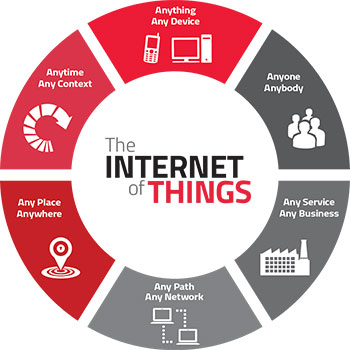
\includegraphics[width=0.4\textwidth]{img/bp/iot-concept.jpg}
    \caption{Internet of Things Networking}
    \label{fig:Figuur8}
    \textit{Source: \autocite{Dauwed2018}}
\end{figure}

%Dankzij de voortdurende innovaties in de technologie hebben de laatste twee decennia een grote invloed gehad op de snelle vooruitgang van IoT. \autocite{Almutairi2024}. Hierdoor is het aantal aangesloten IoT devices sterk gestegen, met 7.74 miljard in 2019, 10.7 miljard in 2021 \autocite{Dawod2022} en tot 75 miljard in 2025 \autocite{Khan2019}. Sensoren, camera's en gelijkaardige apparaten worden al “geïntegreerd” in “woningen” en “voertuigen” \autocite{Dawod2022} en geïmplementeerd over verschillende sectoren zoals de “gezondheidszorg, landbouw, productie transport, milieu en nutsbedrijven \autocite{Naresh2020, Almutairi2024}. De implementatie van miljarden \autocite{Dawod2022} IoT devices over verschillende sectoren geeft een duidelijke representatie van de veranderingen die IoT zal brengen in de manier waarop men leeft, werkt en omgaat met de omgeving \autocite{Almutairi2024}. Dit deel heeft verschillende aspecten van IoT behandeld zoals de oorsprong, het concept en het gebruik. Het volgende deel zal dieper ingaan op de hardwarecomponenten om een beter begrip te verkrijgen in de werking van IoT.

%Deze technologie maakt het mogelijk om IoT in te zetten in verschillende sectoren, zoals transport, slimme steden, nutsbedrijven, milieu, gezondheidszorg en veiligheid. Volgens \autocite{Naresh2020} zal dit leiden tot 75 miljard verbonden IoT-devices in 2025 \autocite{Khan2019}. Dit benadrukt het belang van IoT als een technologie en het gebruik hiervan in diverse sectoren. Dit deel heeft verschillende aspecten van IoT behandeld zoals de oorsprong, het concept en het gebruik. Het volgende deel zal dieper ingaan op de hardwarecomponenten om een beter begrip te verkrijgen in de werking van IoT.

%De afgelopen twee decennia hebben een grote invloed gehad op de snelle vooruitgang van IoT \autocite{Almutairi2024}, hierdoor is het aantal aangesloten IoT devices sterk gestegen, met 7.74 miljard in 2019, 10.7 miljard in 2021 \autocite{Dawod2022} en 25.44 miljard tegen 2030 \autocite{Dawod2022}. Sensoren, camera's en gelijkaardige apparaten worden al “geïntegreerd” in “woningen” en “voertuigen” \autocite{Dawod2022} en geïmplementeerd over verschillende sectoren zoals de “gezondheidszorg, landbouw, productie” en slimme steden \autocite{Almutairi2024}.


%Zoals eerder aangetoond beschikt IoT over verschillende componenten die ervoor zorgen dat deze gegevens kan detecteren en verwerken. In het volgende deel worden deze componenten zorgvuldig geanalyseerd. 

\section{IoT hardware componenten} 
Een IoT-omgeving bestaat uit verschillende kerncomponenten zoals sensoren, actuatoren, microprocessors, en communicatie protocollen. Deze maken het mogelijk dat apparaten slim worden en met elkaar kunnen communiceren \autocite{Abraham2023, Gharde2024}. In de volgende secties worden deze componenten verder behandeld om inzicht te geven in de werking van IoT. De eerste component dat geanalyseerd zal worden zijn de sensoren.

\subsection{Sensors}
Sensoren vormen een essentieel onderdeel van een IoT-systeem en worden gebruikt om chemische veranderingen en anomalieën te detecteren \autocite{Abraham2023, Moyer2019, Sehrawat2019}. Het IoT-systeem wordt compleet wanneer deze gegevens gecombineerd worden met actuatoren, die in het volgende sectie worden besproken. 

\subsection{Actuatoren}
Actuatoren zijn componenten elektrische signalen converteren naar fysieke acties \autocite{Zhang2022} en zo de “fysieke wereld” te beïnvloeden op basis van de verzamelde gegevens \autocite{Moyer2019}. Actuatoren werken in samenwerking met sensoren om een compleet IoT-systeem te creëren. In de volgende sectie wordt het IoT-systeem verder toegelicht door de rol van de microprocessoren te introduceren.

\subsection{Microprocessors}
Microprocessoren spelen een essentiële rol in IoT-systemen. Deze fungeren als de centrale eenheid in een IoT-device en zijn verantwoordelijk voor het verwerken van sensorgegevens, uitvoeren van berekeningen en het besturen van actuatoren \autocite{Abraham2023, James2021}. In de volgende sectie worden de communicatieprotocollen besproken, die een belangrijke onderdeel vormen van IoT-systemen.

\subsection{Communicatie protocollen}
Communicatieprotocollen faciliteren de communicatie tussen twee slimme apparaten. Wat betreft IoT werden er diverse communicatieprotocollen ontwikkeld zoals HTTP, MQTT en XMPP. De keuze hangt af van factoren zoals energie-efficiëntie, veiligheid en kwaliteit van de dienstverlening \autocite{Anitha2022, Jeddou2020}. 


\section{IoT-sensoren: types en beschrijving} \autocite{Moyer2019, Sehrawat2019, Kumar2024, Balogun2017, Meenakshi2020, Tresanchez2018, Shanmugavalli2023, Gala2020, Gade2013, Chidurala2021, Karunarathne2018, Srinivasan2022}

\begin{enumerate}
    \item \textbf{Motion sensor:} Een bewegingsdetector is een IoT-apparaat dat fysieke beweging detecteert en ingezet kan worden voor het detecteren van een inbraak. Zo gebruiken \autocite{Tiong2019} motion sensing in een IoT-gebaseerd beveiligingssysteem.
    
    \item \textbf{Pressure sensor:} Een druksensor in IoT-systemen meet en detecteert kracht en drukte en wordt gebruikt om de bezetting van stoelen en bedden real-time te monitoren.
    
    \item \textbf{Optical proximity sensor:} Wordt gebruikt voor het detecteren van objecten door gebruik te maken van licht zonder fysiek contact.
    
    \item \textbf{Wireless Communication:} Is een belangrijk aspect van IoT. Deze zorgt ervoor dat devices met elkaar kunnen communiceren door data te delen en verzenden.
    
    \item \textbf{Thermal camera:} Thermische camera's detecteren infrarode radiatie van objecten met een temperatuur hoger dan nul graden en kunnen worden ingezet voor het monitoren van niet-intrusieve bezetting.
    
    \item \textbf{Proximity sensors:} Proximity sensoren, meestal gebruikt in de industrie en landbouw, detecteren nabijheid van objecten via elektromagnetische velden.
    
    \item \textbf{Image sensors:} Beeldsensoren gebruiken fotodiodes om licht in een bepaald gebied te detecteren. Deze worden toegepast in medische beeldvorming, digitale camera's, nachtzichtapparatuur  en klantmonitoring in winkels
\end{enumerate}


\section{IoT-sensoren: subtypes en beschrijving}\\

\begin{enumerate}
    \item \textbf{Motion sensor}
    \begin{enumerate}
        \item \textbf{Passive Infrared (PIR) sensors:} Detecteert beweging door veranderingen te waarnemen in infraroodstraling.
        \item \textbf{Microwave:} Deze sensor zendt microgolven uit, de reflectie van deze golven wordt geanalyseerd om beweging te detecteren.
        \item \textbf{Ultrasonic:} Zendt en ontvangt geluidsgolven boven de 20 kHz om beweging te detecteren, samen met de afstand tussen objecten.
    \end{enumerate}
    
    % \item \textbf{Pressure sensor}
    % \begin{enumerate}
        %     \item \textbf{Force-Sensitive Resistors:} Is een low-cost pressure sensor waarbij de weerstand verandert wanneer kracht gedetecteerd wordt.
        %     \item \textbf{Strain Gauge Pressure Sensors:} Meet drukte door de deformatie van een materiaal te detecteren.
        % \end{enumerate}
    
    \item \textbf{Optical proximity sensors}
    \begin{enumerate}
        \item \textbf{Infrared break beam sensor:} Een infrarood emitter en een receiver worden tegenover elkaar geplaatst waardoor er een infrarood licht ontstaat. Wanneer een persoon door het licht gaat, wordt deze onderbroken waardoor er een detectie geactiveerd wordt.
        \item \textbf{Diffuse Reflective Optical Sensor:} \\ Wordt gebruikt voor object -en nabijdetectie. Deze sensoren zenden licht uit en meten het gereflecteerde licht van objecten waardoor ze deze kunnen detecteren.
    \end{enumerate}
    
    \item \textbf{Wireless communication protocol}
    \begin{enumerate}
        \item \textbf{BLE (Bluetooth Low Energy) beacon:} Zijn wireless zenders die unieke identifiers uitzenden.
        \item \textbf{Radio Frequency Identification (RFID):} Bestaat uit een tag, reader en middleware software. Maakt gebruik van radiogolven om data draadloos te verzenden.
    \end{enumerate}
    
    % \item \textbf{Thermal camera}
    %  \begin{enumerate}
        %      \item \textbf{Uncooled thermal camera:} Een device voor het detecteren van infraroodradiatie zonder de nood voor een koelsysteem.
        %      \item \textbf{Cooled thermal camera:} Detecteert infrarode radiatie met hoge snelheid en gevoeligheid door de sensoren naar cryogenische temperaturen te laten dalen.
        %  \end{enumerate}
    
    \item \textbf{Proximity sensors}
    \begin{enumerate}
        \item \textbf{Inductief:} Detecteert geleidende en niet-geleidende materialen door middel van een elektromagnetisch veld.
        \item \textbf{Capacitief:} Maakt gebruik van zwakke elektrische velden om geleidende en niet-geleidende materialen te detecteren.
        \item \textbf{Ultrasoon:} Wordt gebruikt om nabijheid en afstand te meten door middel van een hoogfrequente geluidsgolf.
    \end{enumerate}
    
    \item \textbf{Image sensors}
    \begin{enumerate}
        \item \textbf{Linear image sensor:} Legt lijn voor lijn afbeeldingen vast waardoor real-time tracking van stoelbezetting mogelijk is. Kan in de gezondheidszorg gebruikt worden om de bezetting van wachtruimtes en patiëntenflow te monitoren.
        \item \textbf{Infrared Image Sensors:} Detecteert infraroodradiatie en converteert het naar een beeld.
    \end{enumerate}
\end{enumerate}


\section{Sensoren geschikt voor bezettingsdetectie in wachtruimte}
Op basis van de literatuur zijn er vijf sensortypes geïdentificeerd die relevant zijn voor het meten van bezettingsgraden in wachtruimtes en hun frequente toepassing in de literatuur. De selectie is gebaseerd op hun toepasbaarheid in kleine tot middelgrote ruimtes, real-time mogelijkheden, kost, installatiegemak en privacyvriendelijkheid. In Tabel~\ref{tab:sensorvergelijking} worden deze technologieën vergeleken.

\begin{table}[h!]
    \small
    \centering
    \caption{Overzicht van de voor- en nadelen van sensortypes voor bezettingsdetectie}
    \label{tab:sensorvergelijking}
    \begin{tabular}{|p{2.5cm}|p{3cm}|p{2.8cm}|p{3.4cm}|p{1.9cm}|}
        \hline
        \textbf{Sensor} & \textbf{Voordelen} & \textbf{Nadelen} & \textbf{Privacy\-vriendelijk} & \textbf{Real-time} \\ \hline
        PIR (passieve infrarood) & Goedkoop, laag energieverbruik, vaak gebruikt in smart offices & Detecteert geen stilstand, beperkte nauwkeurigheid & Ja & Ja \\ \hline
        ToF (Time-of-Flight) & Hoge nauwkeurigheid, werkt bij duisternis, geschikt voor afstandsmeting & Duurder, gevoelig voor reflecties & Ja & Ja \\ \hline
        CO₂-sensor & Indirecte bezettingsmeting via luchtkwaliteit, geschikt voor trendanalyse & Trage respons, onnauwkeurig bij kleine groepen & Ja & Nee \\ \hline
        Bluetooth/Wi-Fi tracking & Gedetailleerde gebruikersdata, geschikt voor grote ruimten & Vereist actieve toestellen, privacyrisico’s & Nee & Ja \\ \hline
        Ultrasoon sensor & Simpel, betrouwbaar op korte afstand, ideaal voor doorgangen & Gevoelig voor omgevingsgeluid, beperkte reikwijdte & Ja & Ja \\ \hline
    \end{tabular}
\end{table}


\subsection{Kritische evaluatie van sensoren voor wachtruimtebezetting}

Hoewel verschillende sensoren in de literatuur als geschikt worden aangemerkt, blijkt uit praktijkstudies dat niet elke technologie even betrouwbaar is in een dynamische omgeving zoals een wachtruimte.

\begin{enumerate}
    \item{\textbf{PIR-sensoren:} hoewel goedkoop en energiezuinig, falen bij stilzittende personen of wanneer een persoon zich lange tijd niet beweegt. Hierdoor ontstaat het risico op onderschatting van de bezettingsgraad.}
    \item{\textbf{Ultrasone sensoren:} zijn gevoeliger, maar gevoelig voor geluidsinterferentie (bv. akoestiek of nabijgelegen apparatuur). Bovendien hebben ze een beperkte detectiehoek, waardoor meerdere sensoren nodig zijn voor volledige dekking.}
    \item{\textbf{CO₂-sensoren:} zijn goed voor trendanalyse maar traag en indirect; een plotselinge toename van personen wordt pas na minuten zichtbaar in de metingen.}
    \item{\textbf{Bluetooth/Wi-Fi:} tracking vereist actieve toestellen (bv. smartphone met Bluetooth aan). Hierdoor worden minder digitale gebruikers – zoals oudere bezoekers of kinderen – niet meegenomen, wat leidt tot vertekening.}
    \item{\textbf{ToF-sensoren (Time-of-Flight):} scoren sterk op nauwkeurigheid en zijn onafhankelijk van licht, maar zijn relatief duur en kunnen reflectieproblemen veroorzaken bij glanzende oppervlakken (bv. ramen).}
\end{enumerate}


\section{Implementaties van IoT in wachtruimtes}

\begin{enumerate}
    \item \textbf{Daniele Spoladore et al. (2024) – Italië}
    \begin{itemize}
        \item \textbf{Doelstelling:} Onderzoeken hoe IoT, AI en Virtual Reality een wachtruimte kunnen transformeren in een smart omgeving.
        \item \textbf{Toepassing van IoT:} De Age-IT prototype maakt gebruik van IoT-sensoren, AI en Virtual Reality. Hoewel de autheurs verwijzen naar IoT-sensoren worden de specifieke types niet vermeld.
        \item \textbf{Conclusie:} Dit systeem biedt een significante stap bij het transformeren van traditionele wachtruimtes in een smart omgeving en het omzetten van wachttijden in diagnostische en therapeutische activiteiten.
    \end{itemize}
    
    \item \textbf{M. Ghazal et al. (2015) – Bahrein}
    \begin{itemize}
        \item \textbf{Doelstelling:} Verbeteren van queue management door de servicekwaliteit te verhogen en wachttijden te verminderen.
        \item \textbf{Toepassing van IoT:} Het systeem maakt gebruik van een ESP32-module om live wachtrijgegevens te versturen.
        \item \textbf{Conclusie:} Het systeem functioneert zoals beschreven in de studie.
    \end{itemize}
\end{enumerate} 

\subsection{Vergelijking tussen IoT-oplossingen en Google Vertex AI Occupancy Analytics}
Zowel sensorgebaseerde als vision-gebaseerde IoT-detectiesystemen, zoals Google Vertex AI Occupancy Analytics, bieden mogelijkheden om ruimtebezetting te monitoren. Sensorgebaseerde systemen, zoals PIR-, ultrasone of infraroodsensoren, zijn relatief goedkoop en privacyvriendelijk, omdat ze geen videobeelden gebruiken. Ze functioneren goed bij uiteenlopende lichtomstandigheden, maar zijn gevoelig voor plaatsing en hebben vaak een beperkt detectiebereik. \\

Google Vertex AI Occupancy Analytics maakt gebruik van videobeelden die via een RTSP-stream naar de cloud worden gestuurd, waar AI de beeldverwerking uitvoert. Het systeem kan personen nauwkeurig tellen, zelfs in complexe situaties. Hoewel Google gebruikmaakt van technieken zoals gezichtsvervaging om anonimiteit te garanderen, blijven er privacyvragen bestaan vanwege het cameragebruik en de cloudgebaseerde verwerking. \\

%Daartegenover staan recente systemen waarbij de AI-verwerking lokaal op het toestel gebeurt (edge computing). In zulke oplossingen worden camerabeelden niet doorgestuurd of opgeslagen; enkel het aantal gedetecteerde personen wordt verzonden. Deze benadering is volledig GDPR-compliant en combineert de nauwkeurigheid van beeldherkenning met maximale privacy. Dergelijke edge-AI-oplossingen werden niet toegepast in dit onderzoek, maar tonen wel het potentieel van privacyvriendelijke beeldanalyse zonder cloudverwerking.



%\section{Voordelen en uitdagingen van IoT in de gezondheidszorg}
%In dit deel worden de voor- en nadelen van IoT in de gezondheidszorg opgenomen volgens de literatuur. Hierbij wordt er rekening gehouden met hoe IoT de gezondheidszorg beïnvloedt en hoe deze de gezondheidszorg heeft getransformeerd. In de volgende secties worden eerst de voordelen besproken gevolgd door de uitdagingen die hierbij horen.


%\subsection{Voordelen}
%Door zorgverleners in staat te stellen om IoT te benutten is het mogelijk om “patiëntresultaten te verbeteren, het gebruik van middelen te optimaliseren, de operationele efficiëntie te verhogen, en patiënten in staat stellen actief deel te nemen aan hun eigen zorg wordt mogelijk gemaakt” \autocite{Inzole2024}. Er zijn een onbeperkt aantal mogelijkheden om de gezondheidszorg te verbeteren door gebruik te maken van IoT, hier zijn enkele belangrijke verbeteringen die IoT brengt \autocite{Inzole2024, Abdulmalek2022}. 

%\begin{itemize}
%    \item Beter behandeling van patiënten
%    \item Vroeg opsporen van ziektes
%    \item Kost van behandeling verminderen
%    \item Beter monitoren en beheren van patiënten
%    \item Verhoogd efficiëntie en verbeterde middelen gebruik
%\end{itemize}

%Ondanks de vele voordelen introduceert IoT ook een aantal uitdagingen, deze worden in het volgende sectie besproken. 

%\subsection{Uitdagingen}
%Hoewel IoT belangrijke voordelen levert aan de gezondheidszorg, brengt IoT nog steeds veel problemen met zich mee zoals aangetoond door figuur \ref{fig:Figuur13}. Het analyseren van deze problemen is essentieel voordat IoT geïmplementeerd kan worden om mitigerende strategieën te bedenken zodat IoT op een verantwoordelijke manier kan uitgerold worden. Hier zijn enkele nadelen van IoT in het gezondheidszorgomgeving \autocite{Inzole2024, Abdulmalek2022}.


%\begin{itemize}
%    \item Security
%    \item Privacy
%    \item Interoperabiliteit
%    \item Naleving van regelgeving
%    \item Ethische consideraties
%\end{itemize}

%\begin{figure}[h]
%    \centering
%    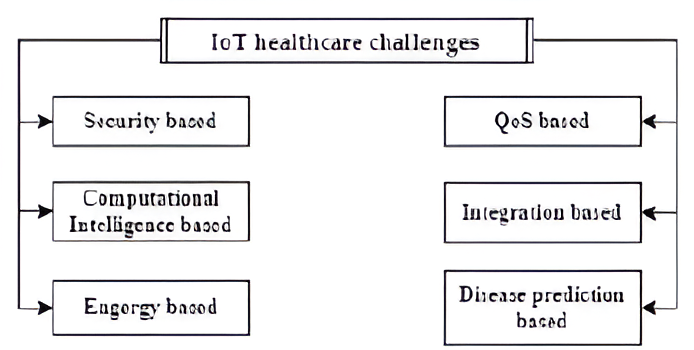
\includegraphics[width=0.60\textwidth]{img/bp/iot-challenges.png}
%    \caption{Nadelen van IoT in het gezondheidszorg}
%    \label{fig:Figuur13}
%    \textit{Source: \autocite{Abdulmalek2022}}
%\end{figure}


%In het volgende deel worden de uitdagingen verder toegelicht, met een specifiek focus op de beveiligings- en ethische kwesties.


%\section{Beveiliging en ethische kwesties van IoT in de gezondheidszorg}
%Met het naadloze integratie van IoT in ziekenhuizen worden patiënten gegevens zorgvuldig verzameld en geanalyseerd waardoor iedere patiënt dezelfde medische diensten kan verwachten. Het gebruik van IoT zorgt ervoor dat patiënten zich niet meer constant hoeven te verplaatsen tussen het ziekenhuis en woonplaats waardoor het niet alleen de sociale lasten maar ook het financiële druk verlaagd \autocite{Chang2019}. Echter, produceren en verzamelen medische instellingen enorme hoeveelheid data (big data) zoals medische dossiers, ziekenhuisdossiers, medische- en biomedische onderzoeksdossiers \autocite{Mirza2022}. Hierbij ontstaan er verschillende beveiligings- en privacy risico's voor patiëntgegevens en vertrouwelijkheid. Deze hebben ernstige gevolgen voor patiënten maar ook voor het vertrouwen in biomedische onderzoeken \autocite{Pandey2018, Juengst2014}. In de volgende sectie worden de beveiligings- en ethische uitdagingen verder in detail uitgewerkt.

%\subsection{Beveiliging} 
%Security problemen zijn een reden voor bezorgdheden vooral door het “enorme snelheid en volumes” waarin medische data wordt gegenereerd. Security wordt gedefinieerd als de “confidentiality, integrity en availability” van het verzamelde data die door het systeem worden verstuurd \autocite{Mittelstadt2017}. Hierbij ontstaan er verschillende security risico's en dit zoals Spoofing, Injection of false signals, Replay attacks, Eavesdropping \autocite{Mirza2022}. Deze risico's ontstaan door “inadequate privacy policies, menselijke fouten, verouderde of onveilige medische apparaten en technologische incompatibiliteit waardoor patiëntengegevens kwetsbaar worden voor misbruik \autocite{Popescul2018}. Ernstige gevolgen kunnen hieruit volgen, waaronder het verlies van mensenlevens, hierdoor wordt security beschouwt als van primordiaal belang \autocite{Ali2024}. Ondanks de uitdagingen dat security met zich meebrengt in IoT is dit niet de enige uitdaging, in het volgende sectie worden de ethische uitdagingen verder besproken.

%\subsubsection{Ethiek}
%Sociale gedrag normen in IoT omvatten beide ethiek en moraal. Ethiek wordt gedefinieerd als hetgeen dat moreel goed of slecht is, en wat fout of juist is, terwijl moraal gedefinieerd wordt als een standaard van normen en regels voor goed gedrag in de samenleving. Ethische gedrag vereist dat men zich houdt aan de volgende richtlijnen \autocite{AboBakr2017, Xhemajli2021}:

%\begin{itemize}
%    \item Privacy van gegevens
%    \item Toegang tot gegevens
%    \item Integriteit van gegevens
%\end{itemize}

%Ethische problemen volgens \autocite{Zakerabasali2022} zijn een van de meest belangrijke en complexe probleem binnen IoT, waardoor het mitigeren hiervan van hoge prioriteit is tijdens de implementatiefase. Figuur \ref{fig:Figuur14} toont de belangrijkste ethische problemen in IoT. 


%\begin{figure}[h]
%    \centering
%    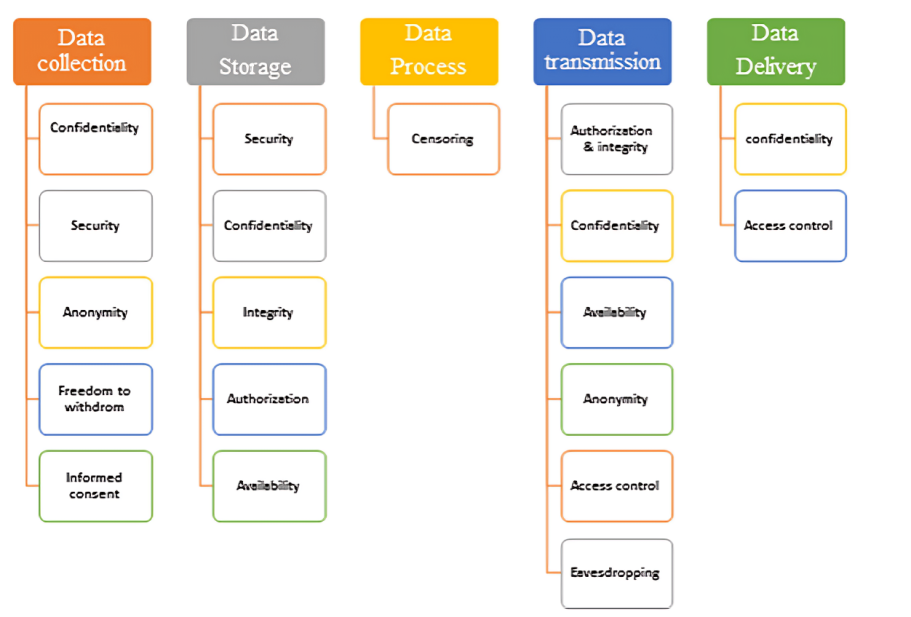
\includegraphics[width=1\textwidth]{img/bp/iot-ethical-issues (1).png}
%    \caption{Ethische kwesties gebaseerd op implementatiefasen van een IoT-systeem.}
%   \label{fig:Figuur14}
%    \textit{Source: \autocite{Zakerabasali2022}}
%\end{figure}

%In het volgende sectie wordt er bekeken naar belangrijke mitigatie strategieën tegen beveiliging en ethische risico's.

%\subsubsection{Mitigatie strategieën}
%De security risico's in IoT kunnen op verschillende manieren gemitigeerd worden zoals het implementeren van “technische maatregelen, policy frameworks en gebruikers educatie”. Deze omvatten de volgende strategieën \autocite{Iwuanyanwu2023}: 

%\begin{itemize}
%    \item Technische maatregelen:“Encryption and Secure Communication, Robust Authentication Mechanism, Software and Firmware Updates en Intrusion Detection Systems (IDS)”
%    \item policy frameworks: “Compliance with Industry Standards and Regulations, Legal Frameworks for IoT Security“
%    \item gebruikers educatie: “Training Programs for End-Users, Promoting Secure IoT Practices”
%\end{itemize}

%De ethische risico's kunnen op diverse manieren worden aangepakt, maar het idee is dat één enkele mitigatie strategie niet genoeg kan zijn om meerdere ethische problemen te behandelen. Daarom wordt er voorgesteld om verschillende strategieën te combineren zoals: 

%\begin{itemize}
%    \item “ethisch gedrag bij het programmeren”
%    \item “whitebox-algoritmen”
%    \item “blackbox-validatie”
%    \item “algoritmische sociale contracten”
%    \item “omhullende IoT-systemen”
%    \item “richtlijnen en ethische code voor IoT-ontwikkelaars”
%%\end{itemize}

%Het combineren van deze strategieën kan ervoor zorgen dat alle aspecten van verschillende ethische risico's behandeld worden \autocite{Loke2019}. Na het bespreken van de beveiliging en ethische kwesties van IoT wordt de focus gelegd op de kern van het onderzoek. In de volgende secties zullen verschillende onderdelen besproken worden die hiermee verband houden. Eerst zullen de wachttijden op de A\&E-afdelingen behandeld worden. Vervolgens zal de impact hiervan op het zorgkwaliteit uitgebreid worden besproken. Tot slot worden de IoT-devices die deze probleem kunnen verhelpen opgesomd en besproken. 

\section{Little’s Law en wachttijdanalyse}
De wet van Little is een fundamentele principe in wachtrij theorie, dat de relatie toont tussen het gemiddelde aantal items of personen in een systeem \(L\), de gemiddelde aankomstsnelheid (\( \lambda \)) en de gemiddelde tijd doorbracht in het systeem \(W\). \autocite{Little2008, Wolff2011}

\[
L = \lambda W
\]

\subsection{Steady-State Aannames voor Little's Law}
Little's Law gaat uit van een steady-state \autocite{Walsh2007} waarbij de aankomstsnelheid gelijk is aan de vertreksnelheid \autocite{Marks2019}. Dit kan problematisch zijn door fluctuaties in het systeem \autocite{Walsh2007} waardoor het moeilijk is om snelheden nauwkeurig te meten \autocite{Hayati2017}.

\subsection{Toepassing van Little’s Law}
Dankzij de eenvoud en brede toepasbaarheid leidt dit tot een wijdverspreid gebruik in verschillende gebieden zoals logistiek en dienstverlening \autocite{SimchiLevi2011}. De veelzijdigheid van de wet komt voort uit vier belangrijke factoren: toepasbaarheid, nut, eenvoud en zichtbaarheid. \autocite{Potter2020}

\subsection{Relevantie voor dit onderzoek}
In dit project vormt Little’s Law het theoretisch kader om de bezettingsgraad te analyseren. Door gebruik te maken van IoT-technologieën kunnen zowel aankomstsnelheid (\( \lambda \)) en verblijftijd (\(W\)) gemeten worden. Daardoor wordt het mogelijk om objectieve berekening van de gemiddelde bezetting (\(L\)) te maakt. Deze inzichten ondersteunen de evaluatie van de impact van het systeem op de wachttijden.  \\ 

Ook in ziekenhuizen en medische praktijken wordt Little’s Law toegepast om het verband tussen patiënteninstroom, verblijfsduur en bezetting te verklaren \autocite{Aahlin2022}. Hierbij wordt het aantal aanwezige patiënten beschouwd als work-in-process binnen het zorgproces, dit geldt ook voor de wachtzaal in dit onderzoek.

\section{Bezettingsdetectie in de praktijk: een overzicht van systemen en studies}
Hieronder worden enkele bestaande systemen en onderzoeken besproken die bezettingsdetectie in de praktijk hebben onderzocht of geïmplementeerd.

\begin{enumerate}
    \item Dit onderzoek stelt een bezettingssysteem voor dat gebruikmaakt van radiogebaseerde frequenties, zoals WiFi en Bluetooth, om de bezetting van een ruimte te detecteren \autocite{Shahbazian2023}.
    
    \item Deze studie onderzoekt en vergelijkt verschillende technologieën voor aanwezigheidsdetectie in gebouwen, met de nadruk op infraroodtechnologieën zoals PIR-sensoren, lichtbarrières en IR-imaging, maar bespreekt ook microgolf- en ultrasoon technologieën. \autocite{Maaspuro2018}
    
    \item Deze studie stelt een deep-learningmodel voor dat op basis van CCTV-beelden zowel het aantal aanwezige personen als hun locaties in gebouwen detecteert. \autocite{Hu2023}
    
    \item De paper onderzoekt hoe een sensornetwerk en machine learning-methodes, zoals Hidden Markov Models, ingezet kunnen worden om bezetting in een open kantoor te schatten op basis van CO₂ en geluid. \autocite{Lam2009}
\end{enumerate}

Op basis van bovenstaande voorbeelden blijkt de combinatie tussen PIR-, ultrasoon- en IR-sensoren een goede balans te bieden tussen nauwkeurigheid, energieverbruik, kostprijs en privacybescherming. Volgens een onderzoek van \autocite{Maaspuro2018} zijn PIR- en ultrasone sensoren zeer effectief in het detecteren van aanwezigheid in gebouwen omdat ze sterk en energiezuinig zijn. In tegenstelling tot methoden op basis van camerabeelden of WiFi/Bluetooth-signalen \autocite{Hu2023, Shahbazian2023}, biedt de IoT-gebaseerde implementatie een eenvoudiger, minder privacygevoelig alternatief dat geen complexe infrastructuur vereist.

\section{Voorspellende modellen op basis van historische data}
Voorspellende modellen worden steeds vaker in verschillende sectoren ingezet om trends in bezoekersaantallen en systeemgebruik te voorspellen \autocite{Ejstrud2006}. Op basis van historische data kunnen algoritmen zoals ARIMA, Random Forest en LSTM-modellen gebruikt worden voor het voorspellen van tijdreeksen, vooral om piekmomenten te identificeren \autocite{Park_2024}. 

\subsection{Praktische toepassingen}
In een aantal onderzoeken wordt de toepassing van ARIMA-, Random Forest- en LSTM-modellen voor tijdreeksvoorspellingen onderzocht, vooral in de context van landbouw en voorraadbeheer \autocite{Nagendra2023}. Deze domeinen tonen het potentieel van dergelijke modellen om processen efficiënter te maken door vooruit te kijken op basis van historische trends.

\subsection{Belang van datakwaliteit en granulariteit}
De effectiviteit van deze modellen wordt sterk beïnvloed door de kwaliteit en kwantiteit van de data \autocite{Mani2021}. IoT-technologieën bieden hierbij een voordeel doordat ze real-time en gedetailleerde gegevens kunnen leveren.

\subsection{Voordeel van voorspellende modellen}
Recent onderzoek toont aan dat het voorspellen van wachttijden en doorlooptijden het middelenbeheer en de klanttevredenheid in verschillende dienstverlenende sectoren aanzienlijk kan verbeteren \autocite{Benevento2021}.

\section{Besluit}
Uit de literatuur blijkt dat IoT-sensoren zoals PIR en ultrasone technologieën zich goed lenen voor bezettingsdetectie in wachtruimtes, vooral wegens hun lage kost, realtime-mogelijkheden en privacyvriendelijkheid. Hoewel systemen zoals Google Vertex AI Occupancy Analytics sterke AI-integratie bieden, brengen ze ook hogere kosten en privacy-uitdagingen met zich mee. Daarom is een eigen Proof-of-Concept met IoT-technologie terecht als praktisch en ethisch alternatief. De toepassing van Little’s Law en voorspellende modellen biedt bijkomende waarde voor capaciteitsbeheer.



% \autocite{Vainieri2020} onderlijnt overbevolking als oorzaak van de hoge werkbelasting, en dit in A\&E departementen in diverse westerse landen. Om beter te begrijpen hoe IoT dit probleem kan oplossen, is het noodzakelijk om dieper in te gaan op wat IoT precies inhoudt. Over het algemeen verwijst Internet of things (IoT) naar een model dat verschillende technologieën omvat. Anders gezegd, is het een netwerk van elektronische apparaten die met elkaar of met de cloud communiceren via het internet. De afgelopen twee decennia hebben een grote invloed gehad op de snelle vooruitgang van IoT \autocite{Almutairi2024}, hierdoor is het aantal aangesloten IoT devices sterk gestegen, met 7.74 miljard in 2019, 10.7 miljard in 2021 \autocite{Dawod2022} en 25.44 miljard tegen 2030 \autocite{Dawod2022}. Sensoren, camera's en gelijkaardige apparaten worden al “geïntegreerd” in “woningen” en “voertuigen” \autocite{Dawod2022} en geïmplementeerd over verschillende sectoren zoals de “gezondheidszorg, landbouw, productie” en slimme steden \autocite{Almutairi2024}.



%\subsection{Implementaties van IoT in wachtruimtes}

%\begin{table}[h]
%    \centering
%    \tiny
%    \caption{Studies: IoT implementaties om wachttijden te verminderen in gezondheidszorg \autocite{Spoladore2024, Ghazal2015}}
%    \begin{tabularx}{\textwidth}{|p{2.5cm}|p{1cm}|p{4cm}|p{4.5cm}|p{3cm}|}
%        \hline
%        \textbf{Author and Year} & \textbf{Country} & \textbf{Objectives} & \textbf{IoT Applications} & \textbf{Conclusion} \\
%        \hline
%        Daniele Spoladore, Marta Mondellini, Atieh Mahroo, Irene Alice Margherita Chicchi Giglioli, Stefano De Gaspari, Daniele Di Lernia, Giuseppe Riva, Elena Bellini, Nicoletta Setola, Marco Sacco   
%        & Italy 
%        & Onderzoeken hoe IoT, AI en Virtual reality een wachtruimte kan transformeren in een smart omgeving. 
%        & De Age-IT prototype maakt gebruik van IoT sensoren, AI en virtual reality.
%        & Dit systeem biedt een significante stap bij het transformeren van traditionele wachtruimtes in een smart omgeving en het omzetten van wachttijden in diagnostische en therapeutische activiteiten. \\
%        \hline
%        M. Ghazal, Rania Hamouda, Samr Ali
%        & Bahrain 
%        & Het doel is om de queue management te verbeteren door de service kwaliteit te verhogen en wachttijden te verminderen
%        & Het systeem maakt gebruik van ESP32 om live queue data te versturen.
%        & Het systeem werkt zoals weergegeven in de studie.  \\
%        \hline
%    \end{tabularx}
%    \label{tab:IoT_waiting_time_reduction_waitingroom}
%\end{table}


%\section{Plaatsing strategieën van IoT}
%De plaatsing van een IoT device wordt gecategoriseerd worden in twee diverse plaatsing strategieën, de fysieke plaatsing en netwerk plaatsen. In de netwerkplaatsing wordt de focus gelegd op de plaatsing van de IoT-gateways. Aangezien deze buiten de scope van het onderzoek vallen, zijn alleen de fysieke plaatsing en relevante aspecten van belang. Deze worden in de volgende sectie verder toegelicht.

%\subsection{Physical placement}
%Fysieke plaatsing is de manier waarop een device “strategisch geplaatst” wordt voor een betere netwerk performantie en dekking \autocite{Xia2018}. Zie tabel \ref{tab:placement_strategies} voor een overzicht van diverse fysieke plaatsing strategieën.

%\begin{enumerate}

%    \item \textbf{Uniform Random Deployment} \\

%    \textit{Doel:} Devices worden random verspreid om dekking te hebben over een gebied. Uniform deployment is een gemeenschappelijke strategie voor het uitrollen van IoT devices en sensoren in een wireless netwerk. \\

%    \textit{Methode:} Devices worden op een uniforme wijze verspreid over een bepaald gebied. \\
    
    %\textit{Voordelen:} Makkelijk te implementeren, maar heeft weinig dekking en is minder veerkrachtig tegen aanvallen.
    
  
  %  \item \textbf{Grid-Based Deployment} \\
   
   % \textit{Doel:} Biedt voorspelbare en gestructureerde dekking voor wireless netwerken. \\
    
    %\textit{Methode:} Devices worden uitgerold in een geometrisch patroon zoals square grids, triangular grids of hexagonal grids om uniforme dekking te realiseren. Square grids bieden betere dekking, terwijl andere vormen voordelen hebben qua end-to-end delay. \\
    
    %\textit{Voordelen:} Voorspelbare en makkelijk te analyseren dekkingsgebieden.
    
    
    %\item \textbf{Cluster-Based Deployment} \\
    
    %\textit{Doel:} Optimalisatie van data-aggregatie en vermindering van energieverbruik. \\
    
    %\textit{Methode:} Devices worden gegroepeerd in clusters, waarbij een centrale node wordt gebruikt voor data-aggregatie en energie-efficiënte communicatie. \\
    
    %\textit{Voordelen:} Vermindert dataredundantie en communicatie-overhead.
    
    
    %\item \textbf{Mobility-Aware Deployment} \\
    
    %\textit{Doel:} Plaatsing gebaseerd op bewegingspatronen van devices of gebruikers. \\
    
    %\textit{Methode:} Devices worden dynamisch geplaatst op basis van voorspelde bewegingspatronen. \\
    
    %\textit{Voordelen:} Vermindert energieverbruik en verbetert plaatsingsefficiëntie.
    
    
    %\item \textbf{Fixed Placement} \\
    
    %\textit{Doel:} Consistente en betrouwbare dataverzameling. \\
    
    %\textit{Methode:} Devices worden permanent geïnstalleerd op vaste locaties, wat zorgt voor een stabiel netwerk en efficiënte middeleninzet. \\
    
    %\textit{Voordelen:} Betrouwbaar en makkelijk te onderhouden.

%\end{enumerate}

%\subsection{Network placement}
%In Netwerk plaatsing wordt de focus gelegd op de plaatsing van de IoT gateways, om kosten te verminderen en performantie te verhogen \autocite{Patil2021, Patil2021a}. Zie tabel \ref{tab:network_placement_strategies} voor enkele praktische voor beelden van Netwerk strategieën.

%\begin{table}[h]
%    \tiny
%    \caption{Network Placement Strategies for IoT Gateways, \autocite{Mnguni2019, Patil2021a, Patil2021, Beuchat2019, Kotagi2017, Nezami2020, Matni2020, Dautov2017}}
%    \begin{tabular}{|p{3.5cm}|p{6.5cm}|p{4.5cm}|}
%        \hline
%        \textbf{Strategy} & \textbf{Description} & \textbf{Benefits} \\ \hline
%        Fixed Gateway Placement & Gateways worden strategisch geplaatst om de dekking te maximaliseren en de netwerk performantie te verbeteren. & Betrouwbare kwaliteit van de service en vermindering van de kosten. \\ \hline
%        Distance-Based Optimization & Gateways worden geplaatst door middel van optimalisatietechnieken zoals Euclidische of Manhattan-afstand om energieverbruik en latentie te minimaliseren. & Efficiënter gebruik van netwerkbronnen en minder energieverbruik. \\ \hline
%        Load-Balanced Placement & Gateways worden geplaatst op basis van de verkeersbelasting. Load balancing is essentieel bij het verbeteren van netwerk performantie en vermijden van congesties. & Consequente verbetering in netwerk performantie en vertraging. \\ \hline
%        Dynamic Gateway Placement & Gateways wijzigen hun positie op basis van veranderende netwerkcondities, zoals gebruikersmobiliteit of variërende dataverkeerpatronen. & Verminderen van de kosten en betere QoS in dynamische IoT-omgevingen. \\ \hline
%        Hierarchical Gateway Deployment & Meerdere niveaus van gateways worden gebruikt om de belasting te verminderen en reactietijd te verhogen. De lagere niveaus verwerken lokaal, terwijl de hogere niveaus verantwoordelijk zijn voor het versturen van data naar de cloud. & Efficiëntere data-agregatie en verminderde latentie. \\ \hline
%    \end{tabular}
%    \label{tab:network_placement_strategies}
%\end{table}


%\section{Evaluatie van software voor IoT-implementaties}
%Diverse software worden gebruikt om communicatie, verwerking, analyse mogelijk te maken in IoT-implementaties. Het doel van deze sectie is om verschillende software te identificeren door diverse studies te verkennen. Het volgende tabel \ref{tab:software_literatuurstudie} toont een overzicht van onderzoeken

%\begin{table}[h]
%    \tiny
%    \caption{Overzicht van onderzoeken naar softwaregebruik in IoT-implementaties, \autocite{Vikash2020}, \autocite{Giacobbe2020}}
%    \begin{tabular}{|p{2.5cm}|p{4.7cm}|p{5.7cm}|p{3.5cm}|}
%        \hline
%        \textbf{Author} & \textbf{Software} & \textbf{Application} & \textbf{Key findings} \\ 
%        \hline
%        Vikash, Lalita Mishra, Shirshu Varma & Apache NiFi & Automatiseert datastroom tussen systemen  & NiFi biedt hoog throughput en lage latency, is ideal voor gebruik met IoT \\ 
%        \hline
%        Vikash, Lalita Mishra, Shirshu Varma & Apache Storm & Verwerken van real-time, unbounded datastreams & Neemt de kortste opstarttijd. \\ 
%        \hline
%        Vikash, Lalita Mishra, Shirshu Varma & Apache Apex & Ondersteunt streams en batch processing voor real-time big data applications & Minst bruikbare solution voor IoT, biedt low throughput, hoog response time, en maximum jitter. \\ 
%        \hline
%        Vikash, Lalita Mishra, Shirshu Varma & Spark Streaming & Verwerkt in real-time batch data door de taken te verdelen over clusters & N.V.T. \\ 
%        \hline
%        Vikash, Lalita Mishra, Shirshu Varma & Apache Flink & Real-time verwerking van batch data door master, slave architectuur te gebruiken voor parallel uitvoer van taken& Minst scalable solution.  \\ 
%        \hline
%        Maurizio Giacobbe, Chakib Chaouch, Marco Scarpa, Antonio Puliafito & InfluxDB & Time series data store voor IoT en real-time analyse & Verzamelt tijdstempels, id's en sensorgegevens zoals temperatuur, helderheid, kooldioxide in smart city-platform. \\ 
%        \hline
%        Robert Stackowiak & Microsoft Azure IoT Suite: Azure IoT Hub & Maakt verbinding en beheer van IoT-devices mogelijk. & N.V.T. \\ 
%        \hline
%        Robert Stackowiak & Microsoft Azure IoT Suite: Azure Digital Twins & Maakt gebruk van ruimtelijke intelligentiegrafieken om een virtuele weergave van de fysieke wereld te maken & N.V.T. \\ 
%        \hline
%        Robert Stackowiak & Microsoft Azure IoT Suite: Azure Stream Analytics & Verwerkt hoge volumes streaming data van devices via SQL queries  & N.V.T. \\ 
%        \hline
%        Robert Stackowiak & Microsoft Azure IoT Suite: Azure Time Series Insights & Maakt de analyse en visualisatie van time series data van IoT-devices.   & N.V.T. \\ 
%        \hline
%        Robert Stackowiak & Microsoft Azure IoT Suite: Azure Databricks & Biedt real-time data verwerking, machine learning en autoscalling van IoT  & N.V.T. \\ 
%        \hline
%        Robert Stackowiak & Microsoft Azure IoT Suite: Azure Data Lake Storage & Azure Data Lake Storage Gen2 combineert de kosteneffectiviteit van Azure Blob Storage met verbeterde functies voor het bestandssysteem  & N.V.T. \\ 
%        \hline
%        Robert Stackowiak & Microsoft Azure IoT Suite: Azure HDInsight & Verwerkt en analyseert big data en ondersteunt diverse open-source frameworks& N.V.T. \\ 
%        \hline
%    \end{tabular}
%       \label{tab:software_literatuurstudie}
%\end{table}



%\subsection{Vergelijking: Traditionele versus IoT-gebaseerde wachttijdsreductie}

% De term 'Internet of Things' is ontstaan in 1999, toen Kevin Ashton, een Britse technologiepionier, verschillende objecten probeerde te verbinden met het internet door gebruik te maken van RFID-tags \autocite{Bassi2013, Rejeb2023}.


%Twintig jaar later wordt IoT ingezet in verschillende sectoren, zoals gezondheidszorg, transport, slimme steden, nutsbedrijven, milieu, veiligheid en nog veel meer. \autocite{Khan2019}


% in het gezondheidszorg wordt IoT gebruikt

%De gezondheidszorg heeft de voorbije jaren een indrukwekkende groei gekend dankzij de vooruitgang in IoT \autocite{Rejeb2023}

% Tip: Begin elk hoofdstuk met een paragraaf inleiding die beschrijft hoe
% dit hoofdstuk past binnen het geheel van de bachelorproef. Geef in het
% bijzonder aan wat de link is met het vorige en volgende hoofdstuk.

% Pas na deze inleidende paragraaf komt de eerste sectiehoofding.

% Dit hoofdstuk bevat je literatuurstudie. De inhoud gaat verder op de inleiding, maar zal het onderwerp van de bachelorproef *diepgaand* uitspitten. De bedoeling is dat de lezer na lezing van dit hoofdstuk helemaal op de hoogte is van de huidige stand van zaken (state-of-the-art) in het onderzoeksdomein. Iemand die niet vertrouwd is met het onderwerp, weet nu voldoende om de rest van het verhaal te kunnen volgen, zonder dat die er nog andere informatie moet over opzoeken \autocite{Pollefliet2011}.

% Je verwijst bij elke bewering die je doet, vakterm die je introduceert, enz.\ naar je bronnen. In \LaTeX{} kan dat met het commando \texttt{$\backslash${textcite\{\}}} of \texttt{$\backslash${autocite\{\}}}. Als argument van het commando geef je de ``sleutel'' van een ``record'' in een bibliografische databank in het Bib\LaTeX{}-formaat (een tekstbestand). Als je expliciet naar de auteur verwijst in de zin (narratieve referentie), gebruik je \texttt{$\backslash${}textcite\{\}}. Soms is de auteursnaam niet expliciet een onderdeel van de zin, dan gebruik je \texttt{$\backslash${}autocite\{\}} (referentie tussen haakjes). Dit gebruik je bv.~bij een citaat, of om in het bijschrift van een overgenomen afbeelding, broncode, tabel, enz. te verwijzen naar de bron. In de volgende paragraaf een voorbeeld van elk.

% \textcite{Knuth1998} schreef een van de standaardwerken over sorteer- en zoekalgoritmen. Experten zijn het erover eens dat cloud computing een interessante opportuniteit vormen, zowel voor gebruikers als voor dienstverleners op vlak van informatietechnologie~\autocite{Creeger2009}.

% Let er ook op: het \texttt{cite}-commando voor de punt, dus binnen de zin. Je verwijst meteen naar een bron in de eerste zin die erop gebaseerd is, dus niet pas op het einde van een paragraaf.

%\begin{figure}
%  \centering
%  \includegraphics[width=0.8\textwidth]{grail.jpg}
%  \caption[Voorbeeld figuur.]{\label{fig:grail}Voorbeeld van invoegen van een figuur. Zorg altijd voor een uitgebreid bijschrift dat de figuur volledig beschrijft zonder in de tekst te moeten gaan zoeken. Vergeet ook je bronvermelding niet!}
%\end{figure}

%\begin{listing}
%  \begin{minted}{python}
%    import pandas as pd
%    import seaborn as sns

%    penguins = sns.load_dataset('penguins')
%    sns.relplot(data=penguins, x="flipper_length_mm", y="bill_length_mm", hue="species")
%  \end{minted}
%  \caption[Voorbeeld codefragment]{Voorbeeld van het invoegen van een codefragment.}
%\end{listing}

%\lipsum[7-20]

%\begin{table}
%  \centering
%  \begin{tabular}{lcr}
%    \toprule
%    \textbf{Kolom 1} & \textbf{Kolom 2} & \textbf{Kolom 3} \\
%    $\alpha$         & $\beta$          & $\gamma$         \\
%    \midrule
%    A                & 10.230           & a                \\
%    B                & 45.678           & b                \\
%    C                & 99.987           & c                \\
%    \bottomrule
%  \end{tabular}
%  \caption[Voorbeeld tabel]{\label{tab:example}Voorbeeld van een tabel.}
%\end{table}

